\documentclass{article}

\usepackage[paper = a4paper, margin = 1in]{geometry}
\usepackage[italian]{babel}
\usepackage[utf8]{inputenc}
\usepackage{hyperref}
\usepackage[T1]{fontenc}
\hypersetup{
    colorlinks=true,
    linkcolor=black,
    urlcolor=blue,
}
\urlstyle{same}

% Math and physic packages
\usepackage{amsmath,amssymb,amsthm}
\usepackage{mathrsfs}
\usepackage{mathtools}
\usepackage{physics}
\numberwithin{equation}{section}

\title{Sviluppo di un sistema di controllo e di acquisizione per sorgente di singolo fotone}
\author{Marco Gobbo, Aurora Perego, Davide Vertemati}

\begin{document}

\maketitle

\section{17 Novembre 2021}
\subsection{Studio dell’apparecchio LDM9LP 
Pigtailed Laser Mount}
Modello: LDM9LP\\
\href{https://www.thorlabs.com/_sd.cfm?fileName=TTN027954-D02.pdf&partNumber=LDM9LP}{Manuale e documentazione forniti da Thorlabs}\\
\href{https://www.thorlabs.com/newgrouppage9.cfm?objectgroup_id=4839&pn=LDM9LP#4839}{Informazioni generali fornite da Thorlabs}

\subsection{Calcolo rate di fotoni}
Formule utili:
\begin{equation} \label{dB}
    1 \text{ dB}_\text{m}=10 \log_{10}\left(P\left[\text{mW}\right]\right)
\end{equation}

\begin{equation*}
    \text{Energia sorgente} [\text{J}] = P[\text{W}]\cdot t[\text{s}]
\end{equation*}

\begin{equation} \label{fotoni}
    \text{Numero fotoni}=\frac{\text{Energia sorgente}}{h\nu}
\end{equation}

\noindent In elettrodinamica classica il valore di aspettazione sul vuoto di $E^2$ è $\bar{n} \frac{\hbar c}{\lambda}$, mentre in QED è $\frac{\hbar c}{\lambda^4}$.
Per questo motivo per apprezzare gli effetti quantistici dobbiamo avere che $\bar{n}\ll\frac{1}{\lambda^3}$. \\
\noindent Il laser utilizzato ha una lunghezza d'onda di $1454.4$nm ($\nu = 2.06 \cdot 10^{14}$Hz) e una potenza di $1.5$mW. Con questi dati calcoliamo il numero di fotoni emessi dal laser in un secondo tramite l'Eq \eqref{fotoni}:
\begin{equation*} 
    \text{Numero fotoni}=\frac{1.5\cdot10^{-3}\text{W}\cdot1\text{s}}{6.626 \cdot 10^{-34} \text{J s} \cdot 2.06 \cdot 10^{14}\text{Hz}} = 1.1\cdot 10^{16}
\end{equation*}
e i decibel-milliwatt della sorgente con l'Eq. \eqref{dB}:
\begin{equation*}
    1 \text{ dB}_\text{m}=10\log_{10}\left(P\left[1.5 \text{mW}\right]\right)=1.76
\end{equation*}

\noindent Per un singolo fotone a $1545$ nm:
\begin{itemize}
    \item Energia = $1.3\cdot10^{-19}$ J
    \item dB = -$158.86$
\end{itemize}

\noindent Raggiungere un singolo fotone al secondo è impossibile con gli attenuatori che abbiamo, ma soprattutto è inutile poiché considerando l'\textbf{efficienza geometrica} ne vediamo ancora meno, quindi il rate diventerebbe troppo basso. 
Facciamo il calcolo per 10 fotoni al secondo:
\begin{itemize}
    \item Energia = $1.3\cdot10^{-18}$ J
    \item dB = -$148.86$
\end{itemize}
L'attenuazione necessaria è quindi $1.76-(-148.86) = 150.62$
L'attenuazione massima a disposizione è di $156$ e corrisponde a circa $3$ fotoni.

\begin{section}{23 Novembre 2021}
\subsection{Cose fatte a lezione}
È stato preparato il cavo che collegherà il diodo al TEC. Per farlo, sono stati utilizzati nove fili di materiale conduttore, che sono stati saldati alla testa della "presa" che andrà poi a inserirsi nell'apparecchio contenente il diodo (usiamo l'ingresso LD connector e non il TEC). I fili sono stati poi etichettati seguendo lo schema in Figura \ref{fig:pin}. In Tabella \ref{tab:pinfunction} sono riportate le funzioni di ognuno dei pin. 
\begin{figure}[h]
    \centering
    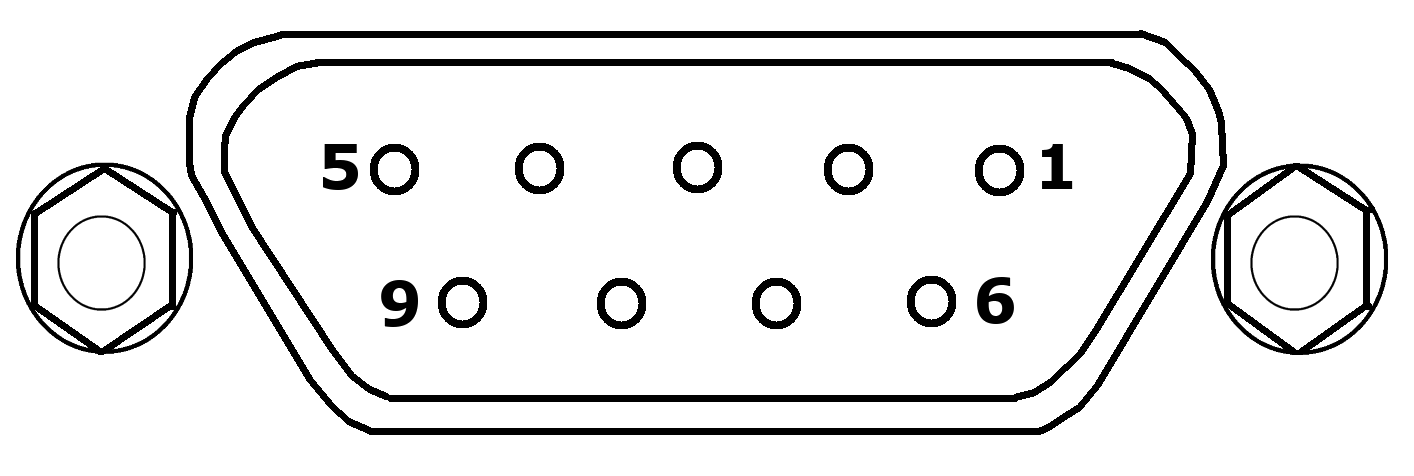
\includegraphics[scale=0.3]{images/pin_scheme.png}
    \caption{Schema della numerazione dei pin del Laser Diode Connector}
    \label{fig:pin}
\end{figure}

\begin{table}[htpb]
    \centering
    \begin{tabular}{c|l}
        \# Pin &	Signal \\
        \hline
        1 &	Interlock and Status Pin (LDC Specific) \\
        2 &	Photodiode Cathode \\
        3 &	Laser Ground (Case) \\
        4 &	Photodiode Anode \\
        5 &	Interlock and Status Return \\
        6 &	Laser Diode Voltage (-) \\
        7 &	Laser Diode Cathode \\
        8 &	Laser Diode Anode \\
        9 &	Laser Diode Voltage (+)
    \end{tabular}
    \caption{Elenco delle funzioni dei singoli pin del Laser Diode Connector}
    \label{tab:pinfunction}
\end{table}

\noindent Infine, i fili etichettati con il numero 9 (l'anodo) e 6 (il catodo) sono stati saldati rispettivamente al centrale (positivo) e alla fascia esterna (negativo) del cavo BNC.

\noindent Per eseguire il collegamento è stata fatta una saldatura fredda: dato che i fili e i pin sono di materiale diverso, sono stati bagnati di stagno prima di essere saldati insieme, in modo tale da creare un sistema che condividesse uno stesso reticolo cristallino e quindi si comportasse allo stesso modo soggetto ad una variazione di temperatura. Infine, le saldature eseguite sul cavo BNC sono state ricoperte da un materiale termorestringente, successivamente riscaldato per mezzo di una HEAT GUN. 

\noindent Durante la fase di collaudo, sono stati testati i vari collegamenti attraverso un generatore di segnale e  sono stati misurati tramite un tester i segnali in vari punti. Il collegamento realizzato con saldature dal generatore al mount del diodo fornisce un segnale, tuttavia il mount con diodo non sembra rispondere a nessuna tensione che viene fornita, nemmeno a quella massima supportata dal dispositivo. Una delle ipotesi di non funzionamento riguarda la configurazione realizzata nel collegamento del diodo al mount, un'altra idea è che il diodo sia già rotto, nonostante sia stato utilizzato un bracciale antistatico durante la fase di collegamento. Si attende una risposta da parte di Faverzani.
\subsection{Materiale utile}
\href{https://www.thorlabs.com/newgrouppage9.cfm?objectgroup_id=1832}{Tutorial diodo laser}\\
\href{https://www.thorlabs.com/newgrouppage9.cfm?objectgroup_id=285}{Fotodiodi}
\end{section}

\end{document}